\documentclass[a4paper,twocolumn]{article}


\usepackage[sc]{mathpazo} % Use the Palatino font
\usepackage[T1]{fontenc} % Use 8-bit encoding that has 256 glyphs
\usepackage[utf8]{inputenc} % Use utf-8 as encoding
\linespread{1.05} % Line spacing - Palatino needs more space between lines
\usepackage{microtype} % Slightly tweak font spacing for aesthetics

\usepackage[spanish]{babel} % Language hyphenation and typographical rules
%\usepackage[galician]{babel} % Change to this if using galician

\usepackage[hmarginratio=1:1,top=32mm,columnsep=20pt]{geometry} % Document margins
\usepackage[hang, small,labelfont=bf,up,textfont=it,up]{caption} % Custom captions under/above floats in tables or figures
\usepackage{booktabs} % Horizontal rules in tables
\usepackage{float} % For [H] float option
\usepackage{abstract} % Allows abstract customization
\renewcommand{\abstractnamefont}{\normalfont\bfseries} % Set the "Abstract" text to bold
\renewcommand{\abstracttextfont}{\normalfont\small\itshape} % Set the abstract itself to small italic text

\usepackage{titlesec} % Allows customization of titles
\renewcommand\thesection{\Roman{section}} % Roman numerals for the sections
\renewcommand\thesubsection{\Alph{subsection}} % roman numerals for subsections
\titleformat{\section}[block]{\large\scshape\centering}{\thesection.}{1em}{} % Change the look of the section titles
\titleformat{\subsection}[block]{\large}{\thesubsection.}{1em}{} % Change the look of the section titles

\usepackage{fancyhdr} % Headers and footers
\pagestyle{fancy} % All pages have headers and footers
\fancyhead{} % Blank out the default header
\fancyfoot{} % Blank out the default footer
%\fancyhead[C]{Running title $\bullet$ May 2016 $\bullet$ Vol. XXI, No. 1} % Custom header text
\fancyfoot[C]{\thepage} % Custom footer text

\usepackage{titling} % Customizing the title section

\usepackage{hyperref} % For hyperlinks in the PDF

\usepackage{graphicx}

\usepackage{amsmath}
 
%----------------------------------------------------------------------------------------
%	TITLE SECTION
%----------------------------------------------------------------------------------------
 
\setlength{\droptitle}{-4\baselineskip} % Move the title up

\pretitle{\begin{center}\huge\bfseries} % Article title formatting
	\posttitle{\end{center}} % Article title closing formatting

\title{Predicción del precio de viviendas residenciales mediante análisis multivariante y técnicas de regularización} % Article title

\author{%
	\textsc{Juan Manuel} \\[1ex] % Your name
	\normalsize Matemáticas y Estadística para la IA\\
	\normalsize Grupo 1 \\ % Your institution
	\normalsize jantofer@myuax.com % Your email address
	%\and % Uncomment if 2 authors are required, duplicate these 4 lines if more
	%\textsc{Jane Smith}\thanks{Corresponding author} \\[1ex] % Second author's name
	%\normalsize University of Utah \\ % Second author's institution
	%\normalsize \href{mailto:jane@smith.com}{jane@smith.com} % Second author's email address
}
\date{\today} % Leave empty to omit a date
\renewcommand{\maketitlehookd}{%
	\begin{abstract}
		\noindent En este caso de uso particular para el conocido dataset "Ames Housing", se realiza una predicción de los precios de viviendas residenciales a través de regresión lineal y técnicas de regularización, que abarca todas las etapas necesarias para la comparación final de la eficacia de los cinco modelos empleados: regresión lineal múltiple con PCA, Lasso, Ridge, y sus versiones con PCA. 
    Para ello, se llevó a cabo un análisis exploratorio de 1460 observaciones y 79 variables predictoras, identificando patrones de correlación con la variable objetivo \texttt{SalePrice} y gestionando los valores ausentes. El preprocesamiento incluyó codificación ordinal y \textit{One-Hot Encoding}, técnicas de imputación de moda y mediana, estandarización y reducción de dimensionalidad mediante PCA. La evaluación final, basada en métricas MAE, RMSE y $R^2$, determinó que el modelo \textbf{Lasso} ofrece la mejor capacidad de generalización, alcanzando un RMSE de \textbf{21771.17} y un $R^2$ de \textbf{0.9327163} en el conjunto de test, demostrando la eficacia de la regularización frente a la alta dimensionalidad. \\\mbox{}\\
		 \textbf{\textit{Palabras clave}: Regresión lineal múltiple, Regularización (Lasso y Ridge), Análisis de Componentes Principales (PCA), Predicción de precios inmobiliarios, R}
	\end{abstract}
}

%----------------------------------------------------------------------------------------

% \begin{document}
	
% 	% Print the title
% 	\maketitle
	
% 	%----------------------------------------------------------------------------------------
% 	%	ARTICLE CONTENTS
% 	%----------------------------------------------------------------------------------------
	
% 	\section{Introducción}
	
% 	Introducción al problema tratado, incluyendo las referencias  necesarias. Por ejemplo: ``Este trabajo se basa en los estudios teóricos realizados en~\cite{Intel:2005} y \cite{spec}". En este apartado se plantean el problema a resolver, objetivos a alcanzar y metodología seguida para alcanzarlos.
	
% 	Es una introducción al problema, no se desarrollarán los contenidos aquí. 
	
% 	La introducción termina indicando en pocas palabras de qué secciones consta el resto del documento y de qué trata cada una. Se mencionan todas las secciones salvo la de referencias (bibliografía). 

% 	%------------------------------------------------
	
% 	\section{Nombre del apartado}
% 	Puede haber tantas secciones como sea necesario para presentar el trabajo pero no más de 4 o 5. Siempre se les pone un nombre que haga referencia al contenido. 
	
% 	Se entra en materia indicando en nuestro caso qué tipo de información vamos a analizar y porqué, así como de donde la hemos obtenido. 
	
% 	Esta sección explica la metodología que hemos usado, por ejemplo el uso de benckmarks, de que tipo son y para que se usan
	
% 	Esta sección puede estar dividida en varias subsecciones. 
	
% 	El cuadro~\ref{tab:valora} muestra un ejemplo de cuadro.
	
% 	Las figuras pueden llevar un encabezado similar o poner el título de la figura al pie de dicha figura. Recordar que todas las tablas y figuras van numeradas para que podamos hacer referencia a ellas en el texto y todas incluyen títulos en los ejes y se indica claramente las unidades de lo representado.
	

% \begin{table}[tb]
% 	{\footnotesize
% 	\caption{Valoración de especificaciones técnicas}
% 	\label{tab:valora}
% 	\centering
% 	\begin{tabular}{|c|c|c|c|c|c|c|}
% 		\hline\hline
% \textbf{TR} & \textbf{INT} & \textbf{ESC} & \textbf{DIS} & \textbf{FIA} & \textbf{TF} & \textbf{MAN} \\\hline
% 5 & 10 & 9 & 7 & 7 & 8 & 3 \\\hline\hline
% \textbf{COM} & \textbf{SEG} & \textbf{COS} & \textbf{TAM} & \textbf{CON} & \textbf{Treal} & \textbf{IS} \\\hline
% 1 & 6 & 5 & 10 & 10 & 2 & 6\\\hline
% 	\end{tabular}
% 	}
% \end{table}
	

	
% %------------------------------------------------
	
% \section{Resultados}
% Se presentan resultados en tablas o en figuras de modo que todas las tablas y figuras tengan un formato similar. Si son datos que nosotros no hemos obtenido, sino que son sacados de libros, artículos o webs debemos indicar la fuente de que fueron obtenidos. Se presentan los resultados.
	
% En los resultados debemos describir cómo hemos realizado los experimentos para que puedan ser reproducidos por terceros. Hay que comentar los resultados antes de pasar a la siguiente sección. 
	
% \subsection{Ejemplo subsección}
% Esta sección puede estar dividida en varias subsecciones. 
	
	
% %------------------------------------------------
	
% \section{Conclusiones}
	
% El apartado de conclusiones explica qué problema ha sido tratado en el documento, qué fue lo que se hizo y cómo se trabajó. Será una especie de recordatorio de todo el documento.

% Se deberán ir desglosando las principales observaciones, conclusiones que podemos extraer y los problemas que se han ido encontrando al ir realizando nuestro trabajo.

% Además, este apartado es el adecuado para exponer cuales podrían ser posibles trabajos futuros que completen lo explicado en este trabajo. 
	


%----------------------------------------------------------------------------------------
%	Referencias
%----------------------------------------------------------------------------------------
	
% \begin{thebibliography}{99} % Bibliografía - alternativamente, se recomienda el uso de bibtex o biblatex
		
% 	\bibitem[1]{Intel:2005}
%     Uhlig, Rich, et al.
% 	\newblock {\em Intel virtualization technology.}
% 	\newblock Computer, vol. 38, no. 5, pp. 48--56, 2005.
% 	\bibitem[2]{spec} Standard Performance Evaluation Corporation, 
% 	\newblock \href{http://www.specbench.org}{http://www.specbench.org}, 	\newblock [online] última visita 20 de marzo de 2017.
		
% \end{thebibliography}
	
	%----------------------------------------------------------------------------------------
	\begin{document}
		% Print the title
		\maketitle
	
		%----------------------------------------------------------------------------------------
		%    ARTICLE CONTENTS
		%----------------------------------------------------------------------------------------
	
	\section{Introducción}
	\label{sec:introduccion}

	La predicción de precios inmobiliarios es un problema fundamental en aprendizaje automático con un gran impacto social y económico, puesto que modelar correctamente el valor de las viviendas ayuda a familias, empresas e instituciones en la toma de decisiones informadas de compra, venta e inversión. Con este fin, este trabajo aplica técnicas de regresión lineal múltiple con regularización a un dataset que contiene viviendas residenciales de Iowa, cada una descrita por 79 variables relativas a ubicación, tamaño, calidad y otros atributos.

	\vspace{0.2cm}
 
	Para la aplicación y evaluación de estos modelos fue necesario realizar: (1) un análisis exploratorio inicial para identificar relaciones con la variable objetivo, \texttt{SalePrice}, (2) el tratamiento de valores nulos según su semántica, (3) la codificación de variables categóricas, (4) la selección y regularización de predictores, y (5) la evaluación comparativa de los enfoques de regresión empleados.

	\vspace{0.2cm}

	Los modelos empleados combinan reducción de dimensionalidad (PCA) y regularización (Lasso $L^1$, Ridge $L^2$) sobre el dataset dividido siguiendo el esquema de particionado 60-20-20. Para la comparación de los mismos, se emplearon las métricas MAE, RMSE y $R^2$, que permiten identificar cuál enfoque logra mejor generalización a precios no vistos.

	\vspace{0.2cm}
	
	El documento está estructurado así: la Sección \ref{sec:eda} presenta el análisis exploratorio y preprocesamiento; la Sección \ref{sec:particionado} explica la división de datos y validación cruzada; la Sección \ref{sec:modelos} describe la construcción de los modelos predictivos; la Sección \ref{sec:resultados} reporta desempeño comparativo; finalmente, la Sección \ref{sec:conclusiones} incluye las conclusiones finales.		%------------------------------------------------



	\section{Análisis exploratorio y preprocesamiento}
	\label{sec:eda}

	\subsection{Objetivo y carga de datos}
		El Análisis Exploratorio de Datos (EDA) permite preparar y manipular los datos de manera óptima para obtener
		respuestas, facilitando la identificación de patrones, la detección de anomalías, y la verificación de hipótesis a
		través de técnicas estadísticas y visuales como gráficos de dispersión, boxplots y matrices de correlación. Esta
		información es fundamental para tomar decisiones sobre el preprocesamiento y la selección de características antes
		de aplicar modelos de ML \cite{eda}.

		\vspace{0.2cm}
 
		El objetivo de este análisis es conocer el conjunto de datos, identificar patrones, tendencias y relaciones relevantes con la variable objetivo \texttt{SalePrice}, y detectar problemas de calidad que condicionen el preprocesamiento y la modelización posteriores. En primer lugar se carga el dataset en un entorno reproducible (en R mediante \texttt{read.csv}) y se realizan operaciones iniciales de inspección: dimensiones, tipos de variables y visualización rápida de filas representativas.

		\subsection{Descripción del conjunto de datos}

		Para comenzar el análisis, se cargó el archivo \texttt{train.csv} mediante la función de R \texttt{read.csv}, y una vez cargado se eliminó la variable \texttt{Id},
		ya que se trata de una variable identificadora y por tanto no aportará a mejorar la predicción de los modelos. 
		
		\vspace{0.2cm}

		El conjunto de datos resultante, definido como \texttt{D}, presenta las siguientes dimensiones tras una inspección inicial realizada a través del comando \texttt{dim}:
		\[
		\mathrm{\dim}(\mathcal{D}) = 1460 \times 80
		\]

		donde $n=1460$ es el número de observaciones (viviendas) y $v=80$ es el número total de columnas, compuestas por 79 variables predictoras y la variable objetivo $Y$ (\texttt{SalePrice}).
		
		\vspace{0.2cm}

		Este primer comando, se ejecutó en la función \verb|inspeccion_rapida()| del script, donde se observa también mediante \verb|str()| y \verb|summary| la coexistencia de tipos de datos heterogéneos
		que muestran la riqueza y variedad de las variables.
		
		\begin{itemize}
			\item \textbf{Variables numéricas:} Incluyen continuas (e.g., \texttt{LotArea}, \texttt{GrLivArea}) y discretas (e.g., \texttt{YearBuilt}).
			\item \textbf{Variables categóricas:} Identificadas en R como \texttt{character} o \texttt{factor}, que requieren codificación posterior (e.g., \texttt{Neighborhood}, \texttt{SaleCondition}).
		\end{itemize}

		\subsection{Análisis de la variable objetivo}
		Como representación inicial, se ha realizado un histograma de la variable objetivo para mostrar su distribución mediante la función \texttt{genero\_histograma},
		que mostró una asimetría positiva, lo que indica que la distribución de sus valores no es normal. Para corregir el sesgo en la visualización,
		satisfaciendo así asunciones de normalidad de los residuos para la confección de los modelos lineales que se verán posteriormente, se aplicó una
		transformación logarítima. La Figura \ref{fig:hist_price} muestra la distribución resultante transformada, generada mediante la función \texttt{hist()} sobre el logaritmo del precio.

		\begin{figure}[h]
			\centering
			% Asegúrate de tener la imagen 'SalePrice_Histograma.png' en tu carpeta
			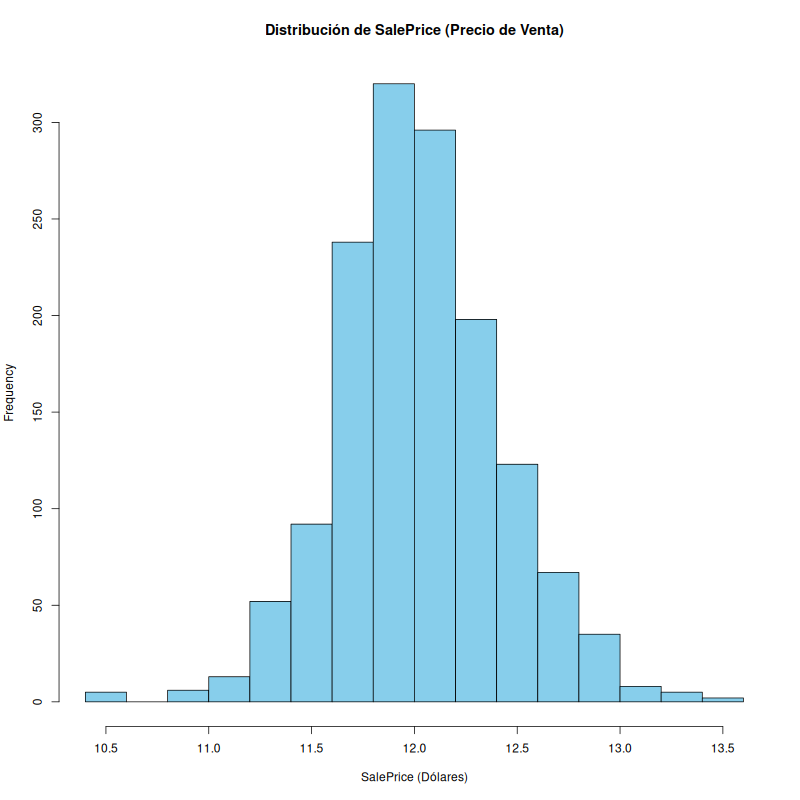
\includegraphics[width=0.8\columnwidth]{SalePrice_Histograma.png}
			\caption{Distribución de la variable objetivo tras la transformación logarítmica.}
			\label{fig:hist_price}
		\end{figure}
		
		Para identificar las relaciones lineales más fuertes entre las variables predictoras y el precio de venta, se ejecutó la función \texttt{analisis\_correlacion} filtrando el dataset para conservar solo las variables numéricas y se calculó la matriz de correlación de Pearson $\mathbf{R}$, utilizando el método \texttt{pairwise.complete.obs} para ignorar los valores ausentes automáticamente, ya que hasta el paso siguiente todavía no fueron gestionados.

		\vspace{0.2cm}

		El script ordena los coeficientes por valor absoluto ($|r|$) para extraer el \textit{Top 15} de variables con mayor influencia lineal sobre el precio. La visualización de estas dependencias se realiza mediante un mapa de calor (\texttt{corrplot}), presentado en la Figura \ref{fig:heatmap}.

		\begin{figure}[h]
			\centering
			% Asegúrate de tener la imagen 'MapaCorrelacion_Predictoras.png' en tu carpeta
			
\includegraphics[width=0.9\columnwidth]{MapaCorrelacion_Predictoras.png}
			\caption{Mapa de calor de las 15 variables numéricas con mayor correlación con \texttt{SalePrice}.}
			\label{fig:heatmap}
		\end{figure}

		Por último, con el fin de detectar valores extremos (outliers) que puedan sesgar los modelos y disparar el error cuadrático medio —métrica que penaliza gravemente las grandes desviaciones al elevar las diferencias al cuadrado—, se realizó una visualización
		con las variables con más influencia en el precio, identificadas anteriormente en la Figura \ref{fig:heatmap}. Como resultado, tras ejecutar la función \texttt{generar\_dispersiones\_top},
		se obtuvo la visualización deseada, como se muestra en Figura \ref{fig:dispersion}. Tras observar cada diagrama de dispersión, es notable de presencia de valores atípicos
		que tienen consecuencias graves en el poder predictivo del modelo, puesto que la variable \textbf{GrLivArea} posee una tendencia de mercado natural, ya que
		a más metros, más cara será la vivienda, pero esto no se cumple en dos valores extremos, puesto que existen dos viviendas con más de 4000 pies con un precio
		a escala logarítima de entre 12 y 12.5, es decir, extremadamente bajo. Lo mismo ocurre con \textbf{TotalBsmntSF}, que denota la presencia de un valor con un sótano enorme
		de unos 6000 pies con un precio muy bajo. Estos valores serán gestionados posteriormente debido a su importancia de cara a la confección del modelo, ya que de no ser así,
		el RMSE penalizará gravemente estos valores y disparará el error de los modelos, cuyo valor ha de ser minimizado y sigue la expresión:

		\[
		\text{Error} = (y_{\text{real}} - y_{\text{predicho}})^2
		\]

		\begin{figure}[h]
			\centering
			% Asegúrate de tener la imagen 'MapaCorrelacion_Predictoras.png' en tu carpeta
			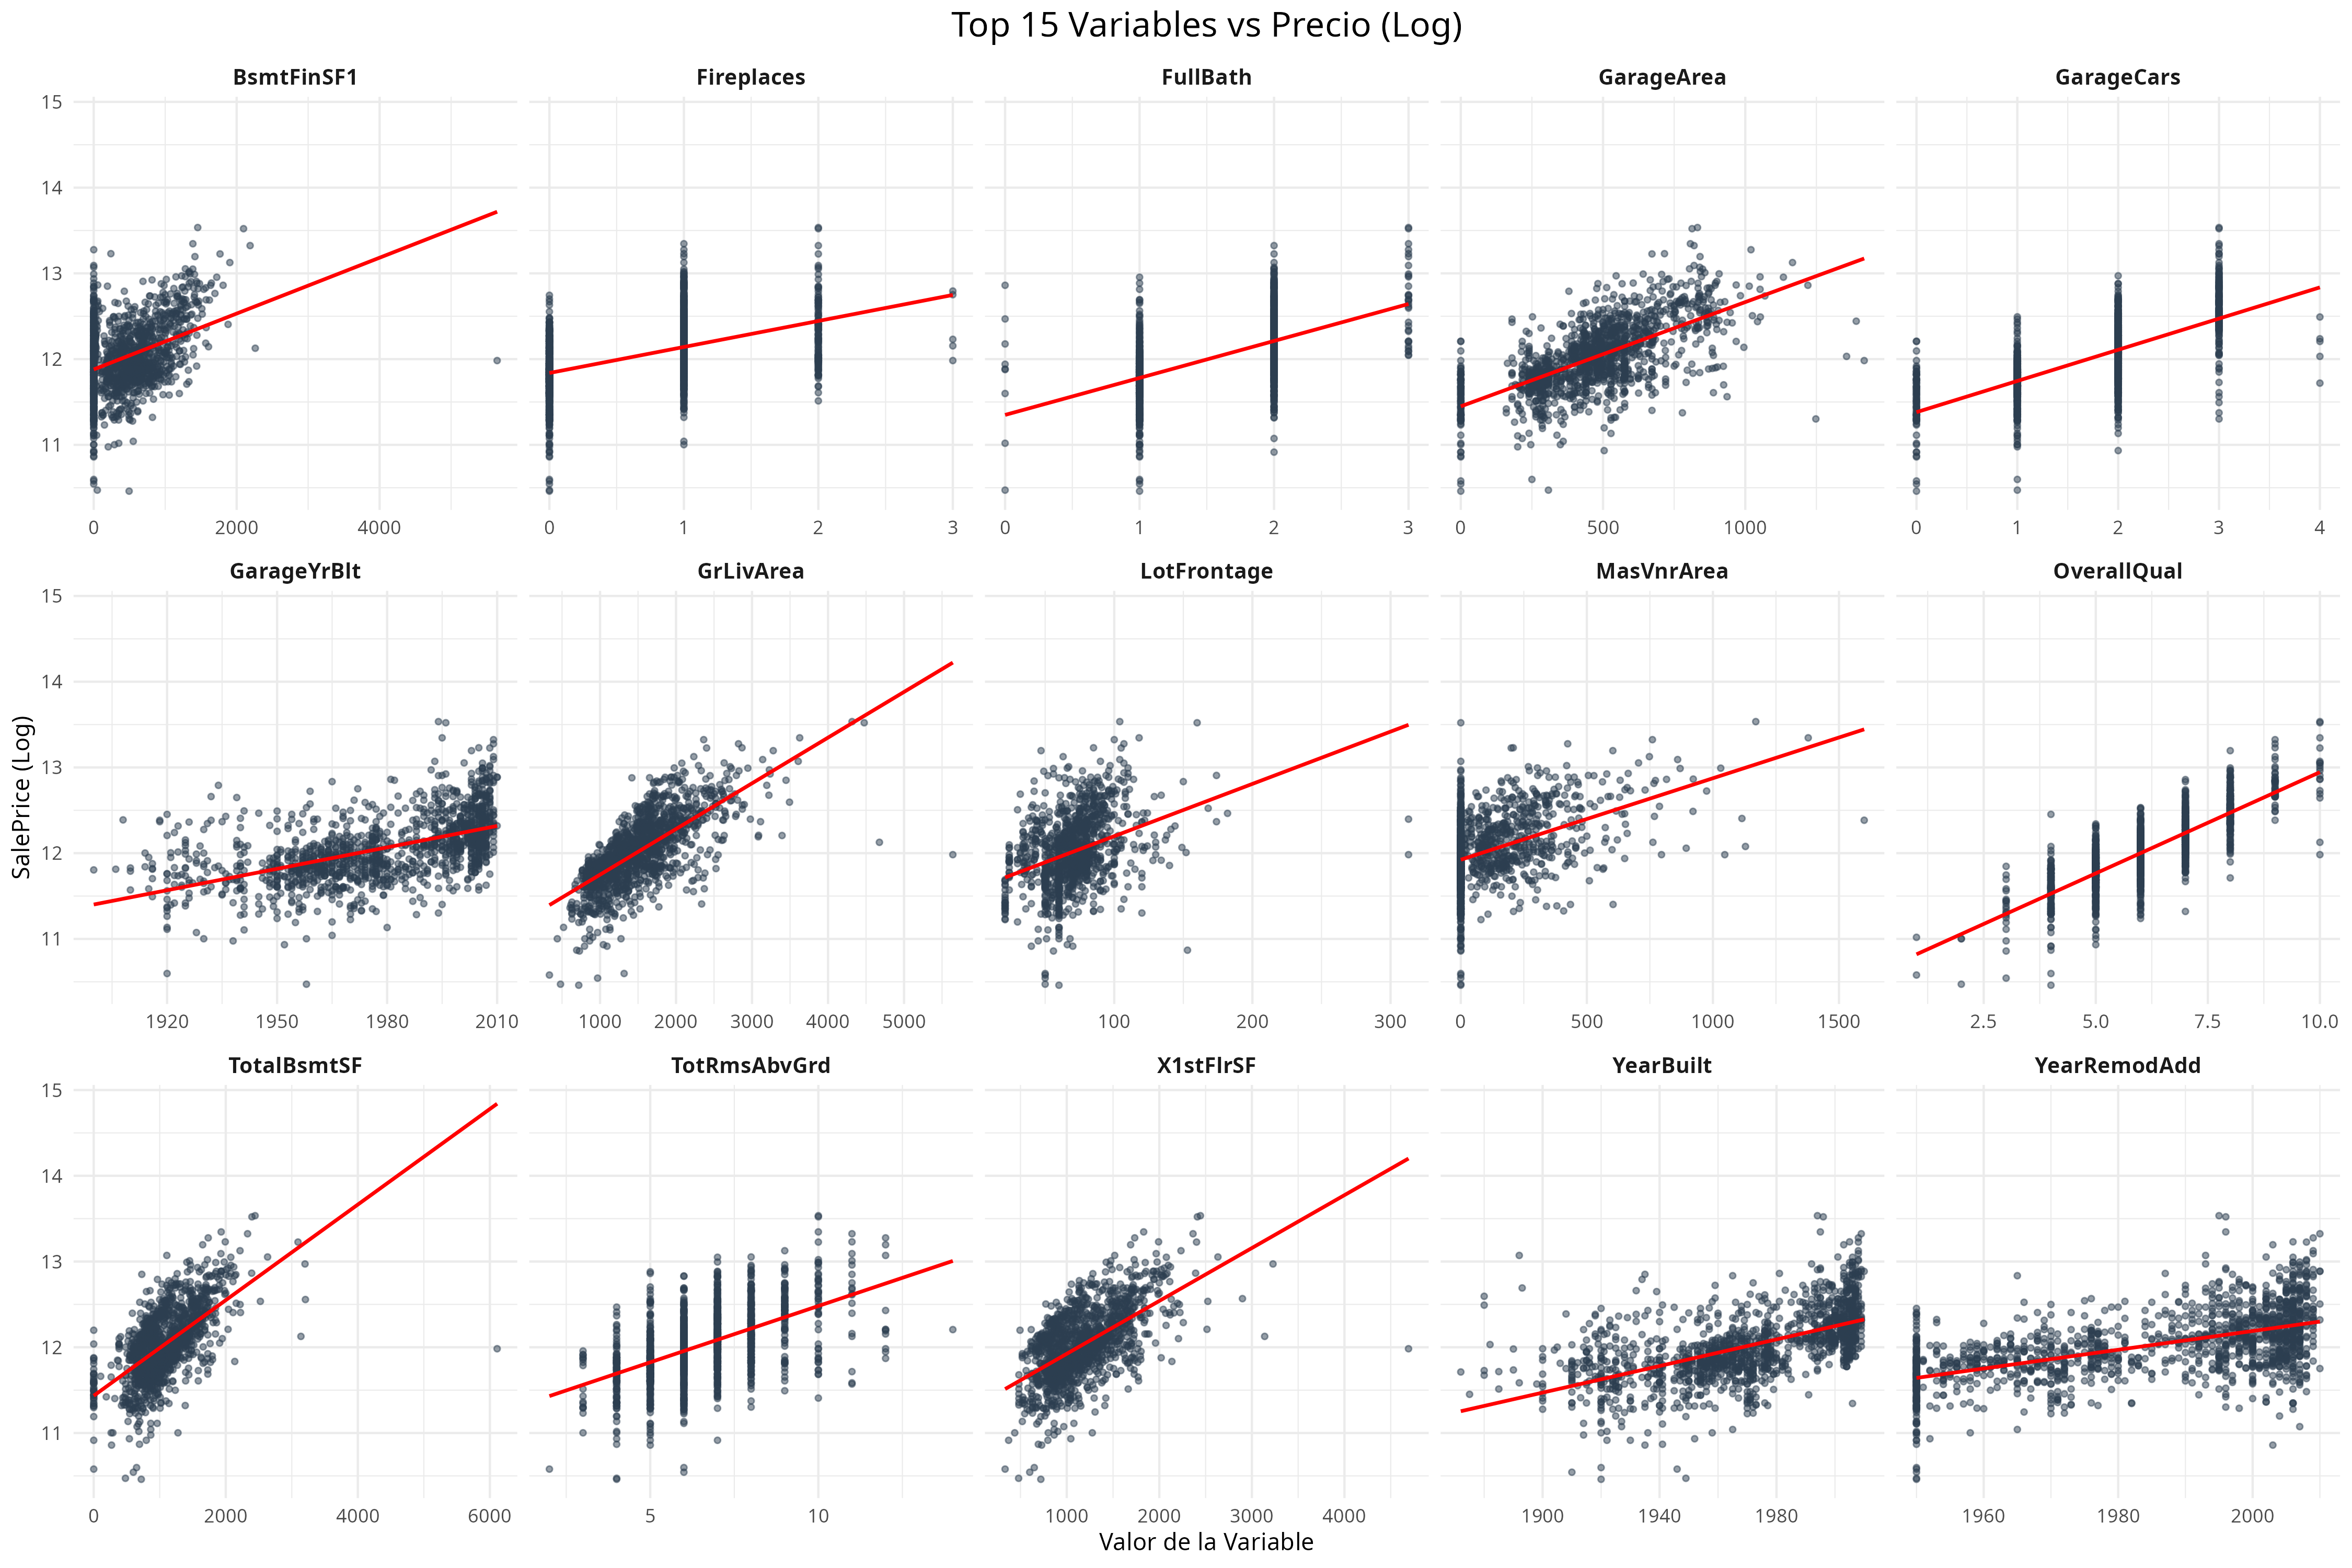
\includegraphics[width=0.9\columnwidth]{Scatterplots_TopVariables.png}
			\caption{Diagrama de dispersión de las 15 variables numéricas con mayor correlación con \texttt{SalePrice}.}
			\label{fig:dispersion}
		\end{figure}

	\subsection{Tratamiento de valores ausentes}
	\label{subsec:valores_ausentes}

	Como se observó en el análisis exploratorio de los datos, existen valores nulos en los mismos, por lo que deberán ser correctamente tratados, ya que el modelo no se puede entrenar con este tipo de valores. Para ello, en primer lugar se calculó el porcentaje de nulos a través de la función \texttt{porcentaje\_nulos}, donde se obtuvieron 19 valores con un porcentaje de valores faltantes mayor que 0, de los cuales cuatro columnas concentran el mayor porcentaje de nulos. 
	
	\vspace{0.2cm}
	
	\begin{figure}[H]
		\centering
		
\includegraphics[width=0.8\columnwidth]{Analisis_Nulos.png}
		\caption{Columnas cuyo porcentaje de nulos es mayor que cero.}
		\label{fig:analisis_nulos}
	\end{figure}
	
	Estos valores identificados, mostrados en Figura \ref{fig:analisis_nulos}, requieren un tratamiento específico basado en su semántica y aporte al modelo, por lo que fue necesario comprender su significado en el fichero \texttt{data\_description}.

	\vspace{0.2cm}

	\subsubsection{Eliminación inicial}

	Una vez realizado un análisis de las variables mostradas anteriormente, se realizó la eliminación de aquellas que no eran relevantes para la confección del modelo, como se muestra en Cuadro~\ref{tab:variables_eliminadas}.

	\begin{table}[tb]
		\centering
		{\footnotesize
		\caption{Variables eliminadas y justificación de su exclusión en el preprocesamiento.}
		\label{tab:variables_eliminadas}
		% CAMBIO AQUÍ: La segunda columna de datos pasa de 'c' a 'p{4.5cm}'
		\begin{tabular}{|l|p{4.5cm}|}
			\hline\hline
			\textbf{Variable} & \textbf{Justificación de eliminación} \\\hline
			RoofMatl & Alta cardinalidad, categorías raras. Dummies esparsas. \\\hline
			Condition2 & Esparsidad extrema: <1\% por categoría. \\\hline
			Exterior2nd & Redundante con Exterior1st. \\\hline
			MiscFeature & >95\% NA, baja varianza. \\\hline
			Alley & ~95\% NA, variable casi constante. \\\hline
			PoolQC & Dominada por NA, poco datos útiles. \\\hline
			Street & ~98\% pavimentadas, variable casi constante. \\\hline
			LandContour & Baja variabilidad, correlación mínima con precio. \\\hline
			LotConfig & Baja importancia predictiva. \\\hline
			Heating & Redundante con HeatingQC. \\\hline
			YrSold & Sin estructura temporal relevante. \\\hline
			MoSold & Estacionalidad inexistente. \\\hline
			Utilities & Casi constante, ~99\% AllPub. \\\hline\hline
			Fence & Alto \% de valores nulos. \\\hline\hline
		\end{tabular}
		}
		\end{table}

	\subsubsection{Tratamiento de las variables}

	En función de la semántica de cada variable, se dividieron los procedimientos aplicados a las mismas en tres tipos, que se incluyen a continuación:

	\vspace{0.2cm}

	\textbf{Ausencia Estructural (Variables Categóricas)} En la gran mayoría de las variables afectadas, el valor NA no indica un dato perdido por error, sino la inexistencia física de la característica en la vivienda (por ejemplo, que la casa no tiene piscina o no tiene garaje).
	\begin{itemize}
		\item \textbf{Variables afectadas:} FireplaceQu, GarageType, GarageFinish, GarageQual, GarageCond, BsmtExposure, BsmtFinType1, BsmtFinType2, BsmtQual, BsmtCond, MasVnrType.
		\item \textbf{Tratamiento:} Se realizó una recodificación explícita, transformando los valores nulos en una nueva categoría denominada \texttt{"None"}.
	\end{itemize}

	\vspace{0.2cm}

	\textbf{Ausencia Estructural (Variables Numéricas)} Son variables asociadas a las anteriores donde la inexistencia del atributo implica una magnitud nula.
	\begin{itemize}
		\item \textbf{Variables afectadas:} GarageYrBlt (Año del garaje) y MasVnrArea (Área de revestimiento).
		\item \textbf{Tratamiento:} Se imputaron directamente con el valor 0 (indicando año 0 o área 0), manteniendo la coherencia con las variables categóricas correspondientes.
	\end{itemize}

	\vspace{0.2cm}

	\textbf{Datos Perdidos Reales} Variables donde la ausencia de información es aleatoria y requiere una estimación estadística para no perder la observación.
	\begin{itemize}
		\item \textbf{Variables afectadas:} LotFrontage (Longitud de fachada, con un 17.7\% de nulos) y Electrical (Sistema eléctrico, con un 0.06\% de nulos).
		\item \textbf{Tratamiento:}
		\begin{itemize}
			\item Para LotFrontage se utilizó la mediana del conjunto de entrenamiento.
			\item Para Electrical se utilizó la moda (valor más frecuente).
		\end{itemize}
	\end{itemize}

	Para evitar la fuga de información (data leakage), estos estadísticos se calcularon exclusivamente sobre el subconjunto
	de entrenamiento (train) y se aplicaron posteriormente a los conjuntos de validación y test, a diferencia de los dos primeros
	tipos de variables tratadas, que al no tener efecto sobre el modelo se realizaron en primera instancia.

	\subsection{Preprocesamiento y codificación}

	El preprocesamiento incluye tres etapas principales ejecutadas tras la partición:

	\vspace{0.2cm}

	\textbf{1. Imputación de valores ausentes:}
	\begin{itemize}
	  \item \texttt{LotFrontage}: mediana del entrenamiento (\texttt{median(..., na.rm = TRUE)}).
	  \item \texttt{Electrical}: moda del entrenamiento (\texttt{sort(table(...), decreasing=TRUE)[1]}).
	  \item Ambas estadísticas se calculan una sola vez con train y se aplican a val y test.
	\end{itemize}

	\vspace{0.2cm}

	\textbf{2. Codificación de variables categóricas ordinales y nominales:}
	Las variables categóricas se codifican en tres grupos mediante funciones personalizadas:

	\begin{itemize}
	  \item \textbf{Ordinales estándar} (calidad con niveles Ex, Gd, TA, Fa, Po): mapeadas a valores numéricos 5, 4, 3, 2, 1 usando \texttt{case\_when()}. Incluyen \texttt{ExterQual}, \texttt{ExterCond}, \texttt{HeatingQC}, \texttt{KitchenQual}, etc.
	  
	  \item \textbf{Ordinales especializadas}: variables con escales personalizadas, por ejemplo \texttt{LotShape} (Reg=3, IR1=2, IR2=1, IR3=0), \texttt{Utilities}, \texttt{LandSlope}, \texttt{Electrical}, \texttt{Functional}, \texttt{PavedDrive}, \texttt{CentralAir}, \texttt{BsmtExposure}, \texttt{BsmtFinType1}, \texttt{BsmtFinType2}, \texttt{GarageFinish}, \texttt{Fence}.
	  
	  \item \textbf{Nominales}: codificación \textit{One-Hot} (dummy variables) mediante \texttt{dummyVars(~ ., ..., fullRank = TRUE)} del paquete \texttt{caret}. Incluyen \texttt{MSZoning}, \texttt{Street}, \texttt{Neighborhood}, \texttt{BldgType}, \texttt{HouseStyle}, \texttt{SaleType}, \texttt{SaleCondition}, entre otras. El parámetro \texttt{fullRank = TRUE} evita la trampa de multicolinealidad eliminando la primera categoría de cada variable.
	\end{itemize}

	\vspace{0.2cm}

	\textbf{3. Estandarización:}
	Las variables numéricas se estandarizan usando \texttt{preProcess(method = c("center", "scale"))} de \texttt{caret}, que:
	\begin{itemize}
	  \item Aprende media y desviación típica del conjunto de entrenamiento.
	  \item Aplica la transformación $z = \frac{x - \mu}{\sigma}$ a todos los conjuntos (train, val, test).
	  \item Es crítico para métodos sensibles a escala (PCA, regularización Lasso/Ridge).
	\end{itemize}

	Tras este preprocesamiento, el dataset está listo para modelado: sin valores nulos, variables categóricas numéricas, y predictores en escala comparable.

	%================================================

	\section{Particionado de datos y validación cruzada}
	\label{sec:particionado}

	Para evitar "data leakage"  se realizó la división del conjunto en subconjuntos de entrenamiento, validación y test \textbf{antes} de aplicar transformaciones que aprendan parámetros del conjunto (imputaciones, escalado, PCA, etc.). La codificación de variables categóricas se realizó en este caso conjuntamente para asegurar la consistencia estructural dimensional, mientras que los parámetros estadísticos se aprendieron únicamente del conjunto de entrenamiento. La disivión se realizó como se muestra a continuación:

	\begin{enumerate}
	  \item Se dividió el dataset completo en train (60\%), validación (20\%) y test (20\%) utilizando \texttt{createDataPartition()} del paquete \texttt{caret}, que realiza un particionado estratificado basado en la variable objetivo.
	  \item Se ajustó todas las transformaciones (imputadores, codificadores, escaladores) únicamente con el conjunto de entrenamiento.
	  \item Se aplicaron las transformaciones aprendidas a los conjuntos de validación y test.
	\end{enumerate}

	\vspace{0.2cm}

	En el script, la partición se realiza mediante:
	\begin{itemize}
	  \item Primer paso: extraer 20\% para test con \texttt{createDataPartition(df\$SalePrice, p=0.2)}.
	  \item Segundo paso: del 80\% restante, extraer 25\% para validación (equivalente al 20\% del total original).
	  \item Resultado: 876 observaciones en train, 292 en validación, 292 en test.
	\end{itemize}

	Esta división garantiza que el modelo generaliza correctamente al no haber visto los datos de validación ni test durante su entrenamiento.

	%------------------------------------------------

	\vspace{0.2cm}

	Por último, como se mencionó anteriormente, existen observaciones de \textbf{GrLivArea} problemáticas, por lo que se estableció un filtro en el dataset que elimina aquellas
	observaciones que tengan un valor de esta mayor a 4000 pies y un precio inferior a 12.5 en escala logarítmica, asegurando así eliminar estos valores conflictivos para el modelo.

	%================================================

	\section{Construcción y evaluación de modelos predictivos}
	\label{sec:modelos}

	Se construyen y comparan cinco modelos de regresión para predecir \texttt{SalePrice}:

	\vspace{0.2cm}

	\textbf{1. Regresión Lineal Múltiple + PCA:}
	
	\vspace{0.2cm}

	Primero se aplica Análisis de Componentes Principales (PCA) al conjunto de predictores estandarizados:
	\[
	\mathbf{PC} = \mathbf{X} \mathbf{W}
	\]
	donde $\mathbf{W}$ son los pesos (eigenvectores) aprendidos únicamente con el entrenamiento. Se seleccionan componentes que expliquen al menos el 95\% de la varianza. Luego se ajusta un modelo lineal:
	\[
	\hat{y} = \beta_0 + \sum_{i=1}^{k} \beta_i \cdot PC_i
	\]
	Este enfoque reduce la dimensionalidad, mitiga multicolinealidad y acelera el cómputo. Se implementa con \texttt{prcomp()} y \texttt{lm()}.

	\vspace{0.2cm}

	\textbf{2. Regresión Lasso:}
	
	\vspace{0.2cm}

	Regularización $L^1$ que añade una penalización proporcional a la suma de los valores absolutos de los coeficientes. La función de pérdida de un un modelo de regresión con regularización $L^1$ se define como:
	\[
	\text{Minimizar:} \quad \frac{1}{2n} \sum_{i=1}^{n} (y_i - \hat{y}_i)^2 + \lambda \sum_{j=1}^{p} |\beta_j|
	\]
	Tiende a forzar algunos coeficientes a exactamente cero, realizando selección de variables automática y se entrena con \texttt{cv.glmnet(..., alpha=1)}, que valida internamente dentro del entrenamiento para encontrar el mejor $\lambda$.

	\vspace{0.2cm}

	\textbf{3. Regresión Ridge:}
	
	\vspace{0.2cm}

	Regularización $L^2$ que penaliza la suma de cuadrados de los coeficientes:
	\[
	\text{Minimizar:} \quad \frac{1}{2n} \sum_{i=1}^{n} (y_i - \hat{y}_i)^2 + \lambda \sum_{j=1}^{p} \beta_j^2
	\]
	Distribuye el peso entre variables correlacionadas, evitando descartes completos. Se implementa con \texttt{cv.glmnet(..., alpha=0)}.

	\vspace{0.2cm}

	\textbf{4. Lasso + PCA y 5. Ridge + PCA:}
	
	\vspace{0.2cm}

	Se aplicaron las regularizaciones Lasso y Ridge sobre los componentes principales en lugar de sobre los predictores originales, combinando así la reducción de dimensionalidad (PCA) con la regularización, con el objetivo de evaluar si dicha combinación mejora la generalización.

	\vspace{0.2cm}

	\textbf{Evaluación y validación cruzada:}
	
	\vspace{0.2cm}

	Cada modelo se entrena con los datos de entrenamiento (60\%) y se evalúa en los conjuntos de validación (20\%) y test (20\%) finales. Las métricas de desempeño son:
	\begin{itemize}
	  \item \textbf{RMSE} (Root Mean Squared Error): $\text{RMSE} = \sqrt{\frac{1}{m}\sum_{i=1}^{m}(y_i - \hat{y}_i)^2}$, donde $m$ es el número de muestras. Penaliza más los errores grandes.
	  \item \textbf{$R^2$ (Coeficiente de determinación)}: $R^2 = 1 - \frac{\sum (y_i - \hat{y}_i)^2}{\sum (y_i - \bar{y})^2}$, porcentaje de varianza explicada.
	\end{itemize}

	Los modelos Lasso y Ridge internamente usan validación cruzada (por defecto 10-fold) con \texttt{cv.glmnet()} para seleccionar automáticamente el parámetro de regularización $\lambda$ óptimo.

	%================================================

	\section{Resultados}
	\label{sec:resultados}

	Para la evaluación de los resultados, se realizó un análisis comparativo de los cinco modelos entrenados, que fueron evaluados en tres fases: entrenamiento en el conjunto de train,
	evaluación preliminar en validación y evaluación final en test.
	Los resultados obtenidos se muestran en Cuadro \ref{tab:resultados}, donde Lasso muestra los mejores resultados, ya que presenta el menor error para el conjunto de test (lo que indica que se acerca más al precio real) y
	tiene el mayor $R^2$, que explica el 93.2\% de la variabilidad del precio. Este modelo ha penalizado aquellas variables que no aportaban al modelo, gestionando correctamente el ruido, por lo que ajustó
	pesos a solo aquellas variables más importantes que permitían la generalización del modelo.

	\vspace{0.2cm}

	Por otra parte, es importante destacar que las versiones de Lasso y Ridge sin realizar una divisón de componentes principales (PCA), muestran unos mejores resultados que sus versiones con dicha
	división. Esto ocurre porque al realizar una reducción de la dimensionalidad se ha perdido información valiosa por el camino, ya que se comprimieron 80 variables en un número muy bajo de componentes.

	\vspace{0.2cm}

	Por último, es notable también el hecho de que no existe overfitting, ya que observando los resultados la diferencia entre el error en validación y el error en test para el modelo ganador es muy baja,
	lo que indica que el modelo no se ha aprendido de memoria los datos, sino que ha logrado generalizar los mismos a partir de su entrenamiento y su ajuste de parámetros.

	\vspace{0.2cm}

	\textbf{Tabla de Resultados Comparativos:}

	\vspace{0.2cm}

	La Tabla \ref{tab:resultados} resume el desempeño de cada modelo en términos de RMSE (validación y test) y $R^2$ en test. En esta tabla, se desestimó el MAE, ya que se consideró que
	el RMSE penaliza más los errores grandes, que son los que más afectan a la predicción del precio de una vivienda. Esta decisión se tomó al considerar que una inmobiliaria prefiere pequeños
	errores constantes a grandes desviaciones puntuales que puedan afectar gravemente a la percepción del cliente.

	\begin{table}[tb]
		\centering
		{\small
		\caption{Comparativa de modelos de regresión: RMSE en validación, RMSE en test y $R^2$ en test.}
		\label{tab:resultados}
		\setlength{\tabcolsep}{4pt}
		\begin{tabular}{|l|c|c|c|}
			\hline\hline
			\textbf{Modelo} & \textbf{RMSE Val} & \textbf{RMSE Test} & \textbf{$R^2$ Test} \\\hline
			OLS-PCA & 21975.54 & 22226.09 & 0.9286668 \\\hline
			Lasso & 20737.97 & 21771.17 & 0.9327163 \\\hline
			Ridge & 21518.62 & 21895.65 & 0.9308782 \\\hline
			Lasso-PCA & 22283.23 & 22444.53 & 0.9297752 \\\hline
			Ridge-PCA & 23182.55 & 24293.32 & 0.9264292 \\\hline\hline
		\end{tabular}
		}
	\end{table}

	%------------------------------------------------

	\section{Conclusiones}
	\label{sec:conclusiones}

	Inicialmente, se realizó un análisis preliminar con motivo de buscar las relaciones entre las variables predictivas y la variable objetivo, atendiendo a la distribución de esta,
	la correlación con el resto, la dispersión entre ellas, así como la mera observación de los estadísticos descriptivos esenciales. Este paso inicial tuvo una gran
	relevancia, al detectar valores nulos que o bien tenían escasa relación con la variable objetivo, o bien no aportaban poder predictivo de la misma.
	A pesar de haber detectado elementos cruciales para la configuración del modelo, fue en la fase final buscando una mejora en los errores cuando se encontraron
	aquellos valores atípicos que más lo disparaban.
	Tras realizar la evaluación de los resultados una vez eliminadas estas observaciones anómalas, fue sorprendente el hecho de cómo varían las métricas finales en función de las decisiones tomadas a lo largo de la confección y ajuste del modelo. Concluyendo
	que la etapa inicial del análisis preliminar de los datos es la más importante a la hora de obtener los mejores resultados, ya que se están empleando técnicas matemáticas que penalizan
	gravemente a aquellos valores de entrada que no siguen fielmente aquellos principios estadísticos que pretenden minimizar o maximizar, y para el cual
	fueron desarrolladas.
	Todo esto proporcionó una comprensión global de cómo los modelos predictivos están condicionados por el cumplimiento de ciertos requisitos de los datos que reciben como entrada. Como
	es el caso del análisis PCA, donde se exigen predictores sin valores nulos, en una escala comparable y con distribuciones simétricas.
	

		%----------------------------------------------------------------------------------------
		%    Referencias
		%----------------------------------------------------------------------------------------
	
		\begin{thebibliography}{99} % Bibliografía - alternativamente, se recomienda el uso de bibtex o biblatex
		    \bibitem[1]{eda} IBM - ¿Qué es EDA?,
		    \newblock \href{https://www.ibm.com/es-es/topics/exploratory-data-analysis}{https://www.ibm.com/es-es/topics/exploratory-data-analysis}, \newblock [online] última visita 27 de noviembre de 2025.
	        
		\end{thebibliography}
	
		%----------------------------------------------------------------------------------------
	
	\end{document}